%%%%%%%%%%%%%%%%%%%%%%%%%%%%%%%%%%%%%%%%%%%%%%%%%%%%%%%%%%%%%%%%%%%%%%
% DelaunayTriangulationSpannerNotes
% March 20th, 2013
% By Simon Pratt (mostly)
\documentclass{tufte-handout}

\usepackage{includes/CGAlgorithms}
\usepackage{includes/QuestionAnswer}
\usepackage{includes/TheoremStuff}
\usepackage{includes/HeaderStuff}
\usepackage{natbib}
\usepackage[pdftex]{graphicx}

%%%%%%%%%%%%%%%%%%%%%%%%%%%%%%%%%%%%%%%%%%%%%%%%%%%%%%%%%%%%%%%%%%%%%%
% Configuration
\newcommand{\DocTitle}{Delaunay Graph Spanner Notes}
\newcommand{\DocAuthor}{Simon Pratt}

\title{\DocTitle}
\author{\DocAuthor}
\fancyhead[L]{\DocTitle}
\fancyhead[R]{\DocAuthor}
\bibliographystyle{plain}

%%%%%%%%%%%%%%%%%%%%%%%%%%%%%%%%%%%%%%%%%%%%%%%%%%%%%%%%%%%%%%%%%%%%%%
% Document
\begin{document}

\maketitle
\vspace{1cm}
% Content starts here

In these notes, we discuss the major results with respect to the
Delaunay Graph as a spanner.

\part{Delaunay Graph}

$P$ is a set of points in the plane, $DG(P)$ is a graph whose vertex
set is $P$ where $u$ and $v$ are connected by an edge only if the
voronoi regions for $u$ and $v$ share an edge.

\begin{figure}
  % http://groups.csail.mit.edu/graphics/classes/6.838/F01/lectures/Delaunay/Delaunay2D.ppt
  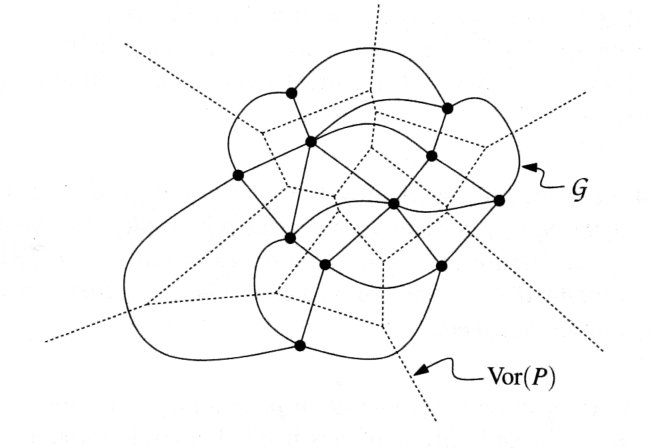
\includegraphics{figures/delaunay_graph.png}
  \caption{The Delaunay graph on $P$, including the boundaries of the
    Voronoi regions.}
\end{figure}

\part{Dobkin's Results}

The Delaunay triangulation of a set of points in the plane is a
spanner with spanning ratio $c \le ((1 + \sqrt{5})/2)\pi \approx
5.08$.  This was proven in the paper ``Delaunay Graphs Are Almost as
Good as Complete Graphs'' by Dobkin, Friedman, and Supowit.  
\cite{Dobkin:1987} \cite{Dobkin:1990}

\section{Introduction}

We consider the path between two arbitray points $a,b \in P$.  Let the
line segment between $a$ and $b$ be the \emph{direct line}.  We
construct \emph{the direct DT path} by walking along the direct line,
each time a new face of the Voronoi diagram is reached we add the
corresponding edge in the Delaunay Graph.

\section{One-Sided Path: The Easy Case}

If all edges along the direct DT path between points $a,b \in P$ are
either all above or all below the direct line, we say that this is a
one-sided path.

\begin{figure*}
  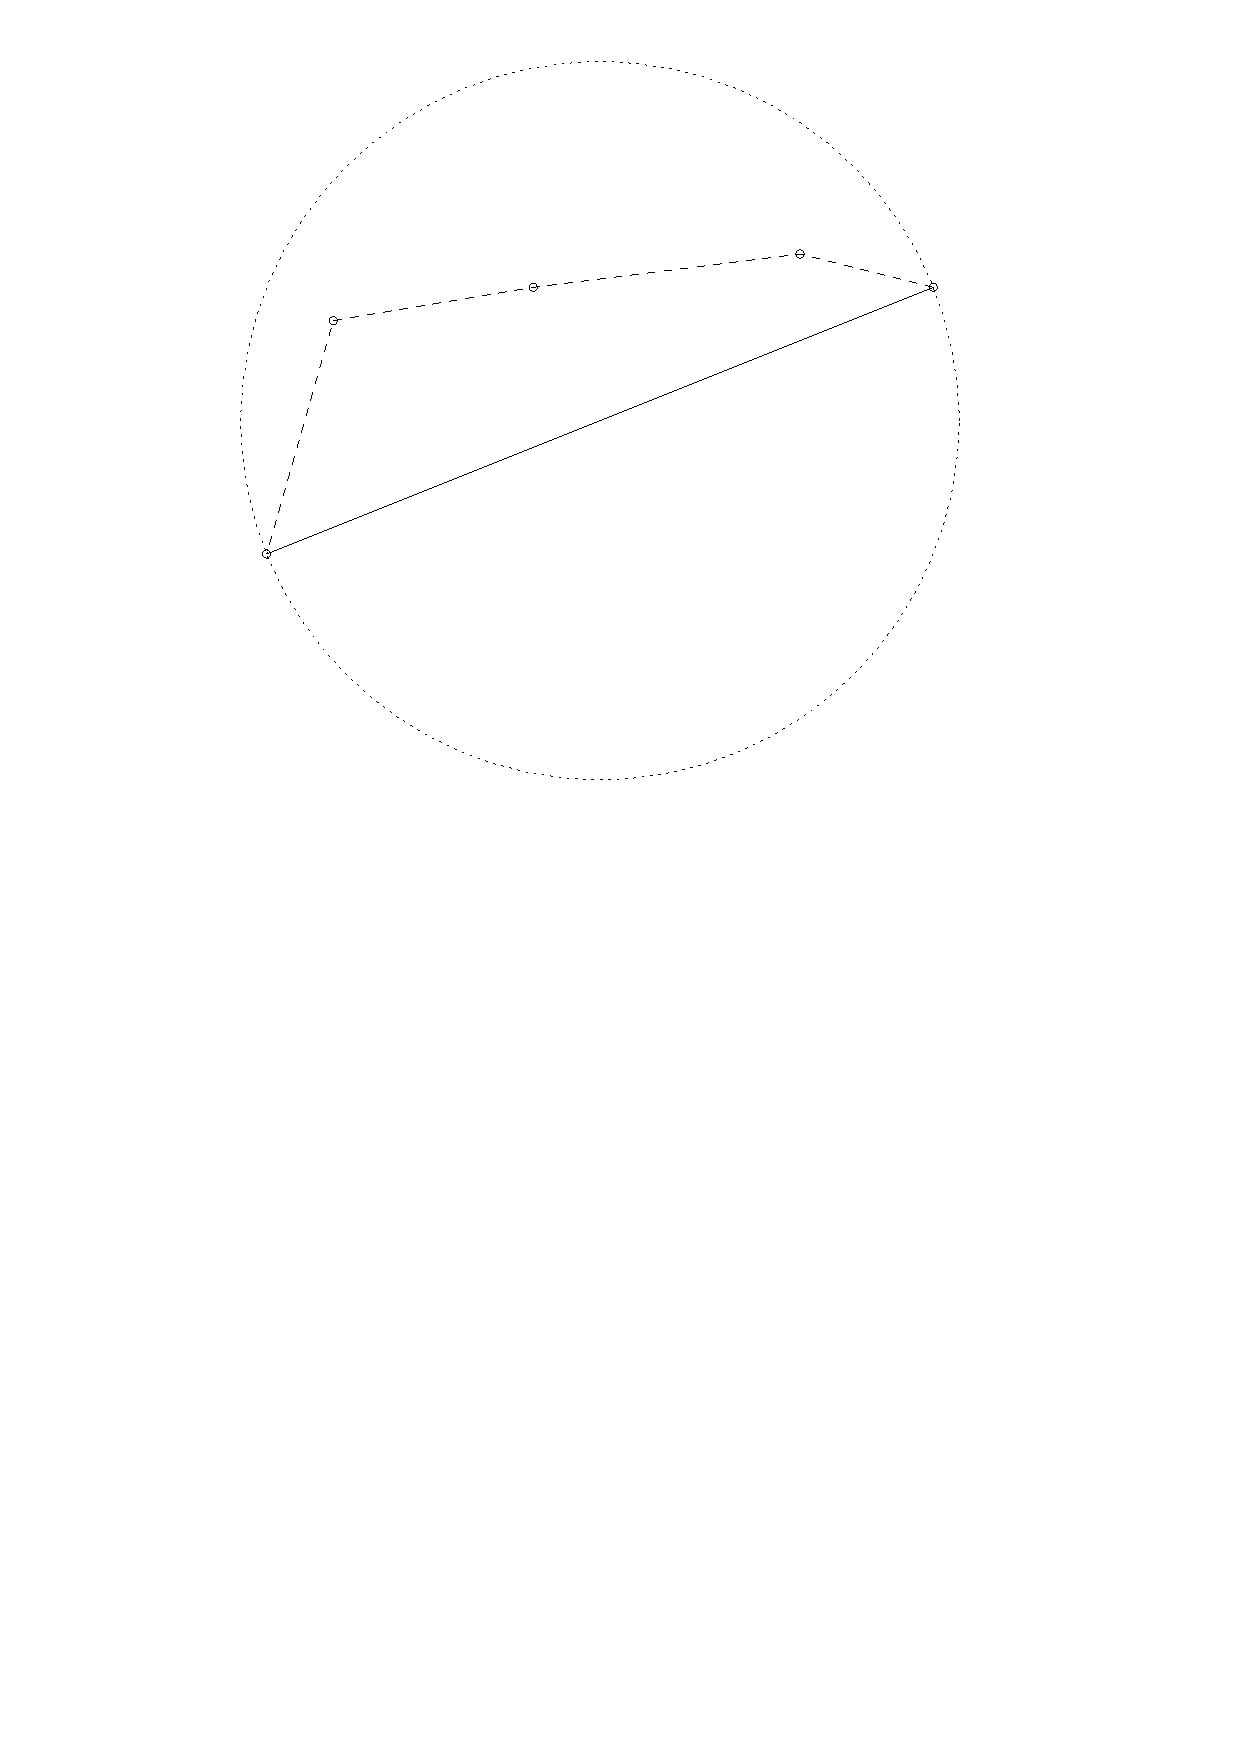
\includegraphics[scale=1.0]{figures/one-sided_path.pdf}
  \caption{The cyan line shows the direct path, the green line shows
    the direct DT path, the dashed red lines show the boundaries of
    the Voronoi regions, and the circumcircles (also dashed) are
    blue.}
\end{figure*}

Without loss of generality, we can say that the line segment between
points $a$ and $b$ lies on the x-axis.

\begin{Lemma}

  Points along a direct DT path are monotonic in $x$.

\end{Lemma}

\begin{Lemma}

  All points along the direct DT path from $a$ to $b$ are contained
  within or on the boundary of the circle with $a$ and $b$
  diametrically opposed.
  
\end{Lemma}

\begin{Lemma}

  The boundary of a connected union of circles has boundary at most
  $\pi \cdot (x_r - x_l)$ where $x_r$ and $x_l$ are the extreme x
  coordinates of any of the circles.
  
\end{Lemma}

From these lemmas, it follows that the one-sided path is at most
$\pi/2$ times as long as the euclidean distance between the endpoints.

\section{The Harder Case}

The direct DT path may cross the x-axis $\BigOmega{n}$ times,
which can yield a much longer path.

\begin{figure}
  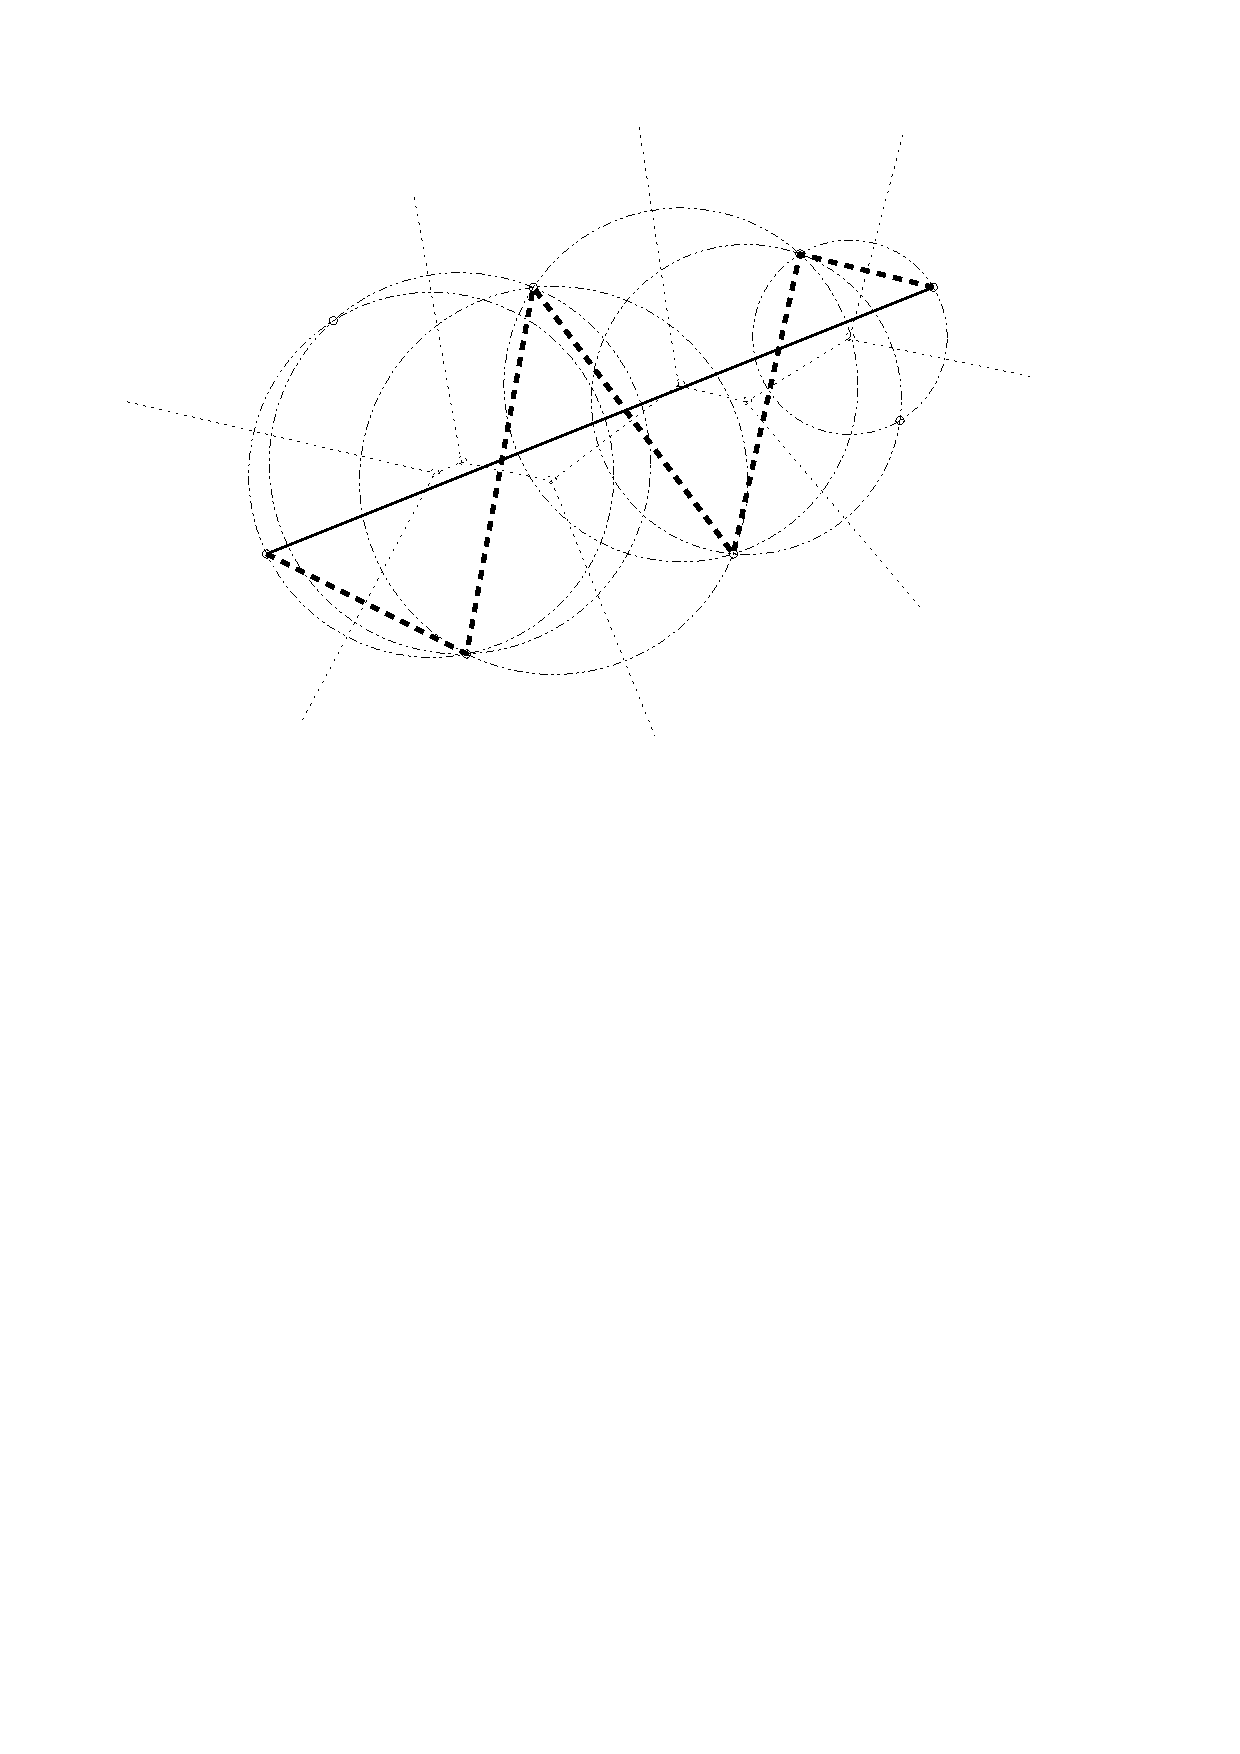
\includegraphics[scale=1.0]{figures/two-sided_path.pdf}
  \caption{A similar diagram with a two-sided direct DT path.}
\end{figure}

The general idea is that we stick to the region above the x-axis as
much as possible, and follow the path below the x-axis if it isn't too
far from the next point above the x-axis. \footnotemark

\footnotetext{
Let $a = p_0, \ldots, p_i, \ldots, p_n = b$ be the direct DT path from
$a$ to $b$.  For each pair $p_i, p_{i+1}$ create the circle on whose
boundary these points lie, and whose centre is on the line segment
between $a$ and $b$.  Let the union of these circles be $T$.

Let $h = min \{ y(q): q \text{ lies on } T \}$, and $w = x(b_j) -
x(b_i)$ where $b_i$ is the last point before the direct DT path dips
below the x-axis and $b_j$ is the first point on or above the x-axis
after $b_i$.  We take the direct DT path only if $h \le w/4$.
}

\begin{figure}
  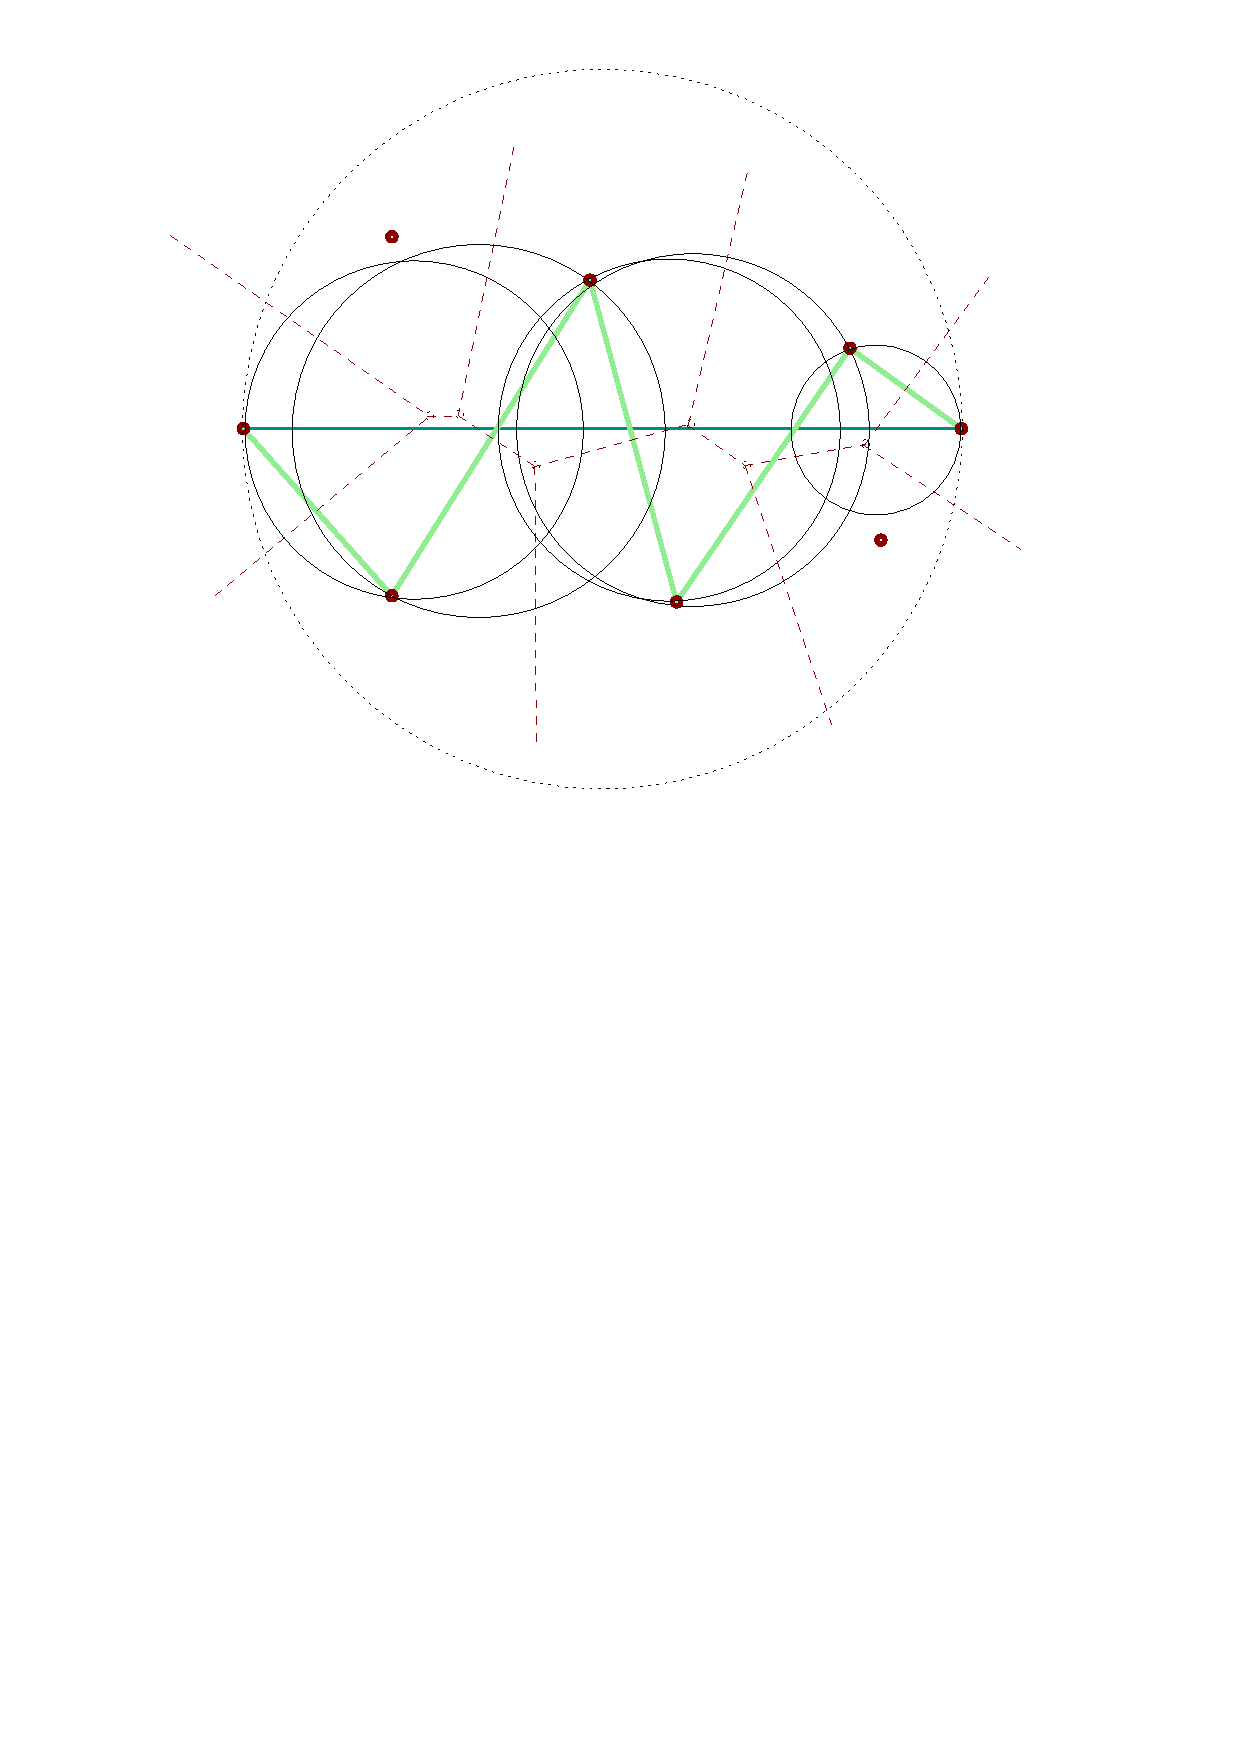
\includegraphics[scale=1.0]{figures/two_sided_path_center_circles.pdf}
  \caption{A two-sided direct DT path showing the circles whose union
    forms $T$ and the dotted circle with $a,b$ diametrically
    oppposed.}
\end{figure}

Otherwise, we follow the lower convex hull of all points in $P$
between $b_i$ and $b_j$, who are above the x-axis and below the line
segment between $b_i$ and $b_j$.

\newpage
\part{Keil's Results}

TODO

% Content ends here

\newpage

\bibliography{references} % uncomment line to add references

\end{document}
